\documentclass[pdftex,12pt]{artikel3}
% Compile with:  pdflatex 

% Settings for source listings.
\usepackage[dvips,letterpaper,margin=1.1in]{geometry}
\usepackage{listings,graphicx}
\usepackage{url}    % usage \href{}{}
\usepackage{xcolor}
%% \usepackage{soul}
%% \usepackage{lipsum}
\usepackage{mathtools}
% \newcommand{\myul}[2][black]{\setulcolor{#1}\ul{#2}\setulcolor{black}}
\usepackage{array}
%% \usepackage{multirow}
\usepackage{alltt}
\usepackage{pifont}
\usepackage{courier}
\usepackage{fancyvrb}
\usepackage{enumitem}
\usepackage[hidelinks]{hyperref}   % hide links in hyperref text
\usepackage{cleveref}     % nice table/figure refs. put after hyperref

% sample stuff for tables and figs
%\usepackage{blindtext}

\usepackage{makeidx}      % for makeindex
\usepackage{tocloft}      % for nicely formatted toc, tof, lof
\usepackage{booktabs,longtable,tabu}

\usepackage[utf8]{inputenc}
\usepackage[T1]{fontenc}
\usepackage{imakeidx}


\usepackage{listings}
\usepackage{color}

\definecolor{dkgreen}{rgb}{0,0.6,0}
\definecolor{gray}{rgb}{0.5,0.5,0.5}
\definecolor{mauve}{rgb}{0.58,0,0.82}

\lstset{frame=tb,
  language=Java,
  aboveskip=3mm,
  belowskip=3mm,
  showstringspaces=false,
  columns=flexible,
  basicstyle={\small\ttfamily},
  numbers=none,
  numberstyle=\tiny\color{gray},
  keywordstyle=\color{blue},
  commentstyle=\color{dkgreen},
  stringstyle=\color{mauve},
  breaklines=true,
  breakatwhitespace=true,
  tabsize=3
}

%% preamble

% the tabfigref command outputs a table or figure reference
% with pattern: "Figure N, The Caption," or "Table N, The Caption,"
% Note: output has a trailing comma(,) for phrasing.
\newcommand{\tabfigref}[1]{\autoref{#1}, \nameref{#1},}

\setcounter{tocdepth}{3}
\makeindex[columns=2, title=Index, intoc]

\lstset{tabsize=4,language=Python,showstringspaces=false}

\title{
\begin{center}
\huge{Jupyter Notebook User Document} \\
\huge{Progessional Communications}\\
\newline
\huge{Team: Dolphins}\\
\end{center}
\\
\\
\\
\\
\author{} % \author{Jeffery B. Russell} \\
          % \author{Dan Moore}
\date{}   % \date{Febuary 20, 2020} 
}

%% document starts
\begin{document}
\maketitle


\begin{center}

\author{Jeffery B. Russell},
\author{Daniel Moore},
\author{Louden Yandow}

\date{March 2, 2020}
\end{center}

\newpage

\tableofcontents
\addtocontents{toc}{~\hfill\textbf{Page}\par}
\addcontentsline{toc}{section}{\listfigurename} % include lists of figs
\newpage
\listoffigures
\addtocontents{lof}{~\hfill\textbf{Page}\par}

\newpage

\section{Introduction}

Jupyter \index{jupyter} is an open-source web-based notebook tool that you can use as your development environment.
A coding notebook enables you to intermix markdown and code blocks that you can execute in a single document. This is heavily used in education and research fields because it makes writing reports easy and reproducible. With Jupyter you can create content that has live code, equations, visualizations and explanatory text. Jupyter is a 

Jupyter Lab extends the basic Jypyter notebook functionality and provides you a full web environment to work in. Using this interface you can open terminals, manage files, and even tile multiple editors.

Applications of Jupyter Jab:

\begin{itemize}
  \item Quick experimentation
  \item Writing a report
  \item Sharing code snippets for education
  \item Generating graphics
\end{itemize}

This document goes over the basic installation and usage of Jupyter Lab for personal development. 
In the advanced usage section we go over how to use Jupyter\index{jupyter} on a remote server. 

\section{Installation}

Full installation instructions can be found on the Jupyter website. \footnote{\url{ https://jupyterlab.readthedocs.io/en/stable/getting_started/installation.html}} This user document goes over how to install Jupyter Lab.

\subsection{Prerequisites}
In order to install Jupyter Lab, you must have Python installed. Your version of Python \textbf{must be 3.3 or greater}. 
As part of having Python, you will also need to have PIP. Although PIP usually comes with your Python installation, there are some exceptions on Linux where you have to install the two seperately.
Go to the Python\index{python} website\footnote{\url{ https://www.python.org/downloads/}} to download the latest version of Python.


We highly recommend you take the time to install \href{https://docs.conda.io/projects/conda/en/latest/user-guide/install/}{Conda}\index{anaconda} because it will be helpful later on with some of the more advanced features of Jupyter as well as machine learning in Python.


You should also have either Firefox, Chrome, or Safari because these are the only browsers Jupyter\index{jupyter} is currently known to work well with.

\subsection{Installation on Linux}
There are two ways of installing Jupyter on Linux.\\
\\
Using pip\index{pip}, the command is:.\\
\begin{lstlisting}
$pip install jupyterlab
\end{lstlisting}

\\
Using conda, the command is:
\begin{lstlisting}
$conda install -c conda-forge jupyterlab
\end{lstlisting}

\subsection{Installation on Windows}
Installation on Windows is the same as installation on Linux except that you must also use the flag to install at a user level if you don't want to run the command as an administrator:
\begin{lstlisting}
>pip install jupyterlab --user
\end{lstlisting}

\section{Usage}

To run Jupyter Lab, open your computer's command terminal and enter the following command. This will open Jupyter Lab in your default web browser.

\begin{lstlisting}
jupyter lab
\end{lstlisting}

Figure 1 is what you will see upon first running Jupyter Lab. Otherwise, it will open to the most recent notebook you were working on.

\begin{figure}[h!]
    \centering
    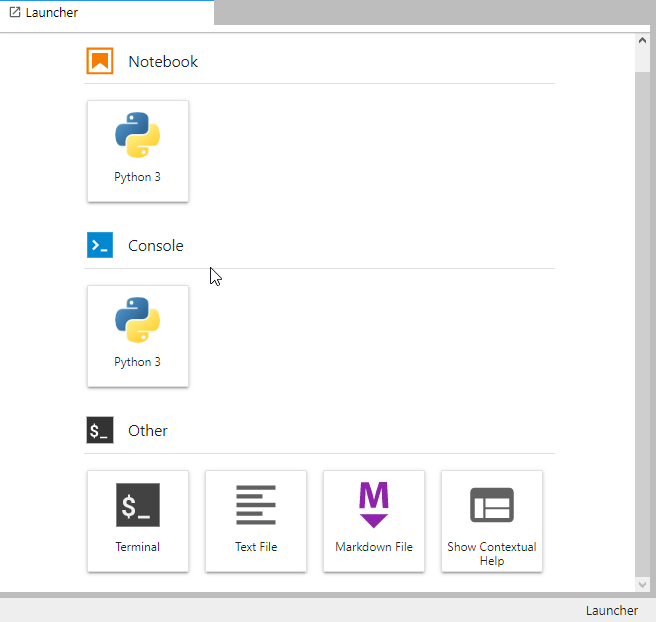
\includegraphics[width=65mm]{launcher.png}
    \caption{Default Jupyter Lab launcher}
    \label{fig:jupyterlablauncher}
\end{figure}

\subsection{Navigation}

Once Jupyter Lab is running, you will see on the left side of the window a column of icons. 
Each icon will open a different panel to the right when clicked. 

\begin{itemize}
    \item File Browser (folder icon): displays a file browser for the user to open, move, or delete their files.
    \item Running Terminals and Kernels (square stop button): shows the user all currently active terminal and kernel sessions.
    \item Commands (palette icon): allows the user to enter various commands into Jupyter Lab.
    \item Notebook Tools (wrench icon): shows various options for the user's current notebook.
    \item Open Tabs (a tabbed window icon): lists all currently open tabs in Jupyter Lab.
\end{itemize}

Additionally, the top toolbar contains the following different drop-down menus: "File", "Edit", "View", "Run", "Kernel", "Tabs", "Settings", and "Help".

\subsection{Creating a Notebook}

To create a notebook from the launcher (figure 1), click on the Python 3 icon under the orange notebook symbol. Alternatively, if you don't have the launcher open, you can click on "File" in the toolbar, click "New", and finally click "Notebook".

This will open an empty, untitled notebook. If you right click on the tab above, or on the name of your notebook in the "Open Tabs" panel on the left, you can rename your notebook.

\subsection{Running a Notebook}

With a notebook open, you can start writing in the editor-- the big empty area on the right half of the screen. Just above the editor, you will find the icon to save the open notebook.

There are also a number of icons that directly relate to the cells you are modifying. A cell may contain either Python\index{python} code, markdown\index{markdown}, or raw text. You can change what type of text a cell is by clicking on the drop-down menu just above the editor that will say either "Code", "Markdown", or "Raw".

The icons above the editor, from left to right, do the following things: 

\begin{itemize}
    \item Add a cell after the currently selected cell.
    \item Cut the currently selected cell.
    \item Copy the selected cell.
    \item Paste the cell from the clipboard.
    \item Run the selected cells and advance to the next cell.
    \item Interrupt the kernel.
    \item Restart the kernel.
\end{itemize}

The following example shows how to write code, run code, and insert raw text into the notebook. First, write some python code and click the "Run selected cells and advance" button (circled in red in the figure below). Our output is shown in figure 2. When a notebooks runs all cells, it executes top to bottom.

\begin{figure}[h!]
    \centering
    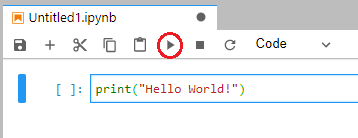
\includegraphics[width=15cm]{code_before_running.png}
    \caption{Code before being run}
    \label{fig:codebeforerunning}
\end{figure}

\begin{figure}[h!]
    \centering
    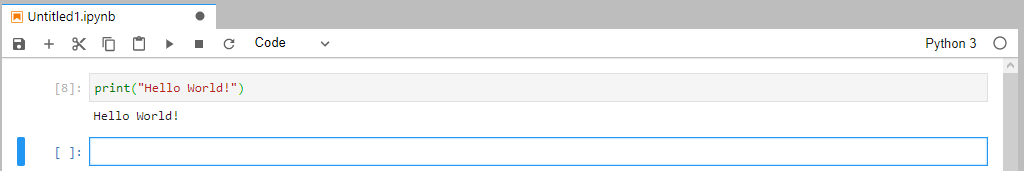
\includegraphics[width=15cm]{code_after_running.png}
    \caption{Code after being run}
    \label{fig:codeafterrunning}
\end{figure}

You can also insert raw text into your document, as shown below.
To do this, change the drop-down menu from "Code" (or "Markdown") to "Raw", and type what you want in the cell.
This is demonstrated in figure 4.


\begin{figure}[h!]
    \centering
    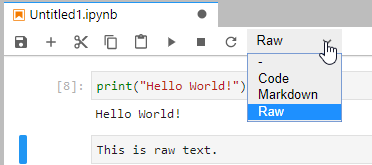
\includegraphics[width=15cm]{raw_text_example.png}
    \caption{Example of raw text}
    \label{fig:rawtextexample}
\end{figure}

\subsection{Exporting Notebooks}
In order to export the document, click the \textbf{File} tab, mouse down to \textbf{Export Notebook As...} and then click a desired format-- Jupyter supports a lot of format types.
The most popular export formats are PDF, Markdown\index{markdown}, and HTML. 

\subsection{Customization}
In general, customization of Jupyter easy.\\
\\
To change the Jupyter theme, go to the "Settings" tab and drop down to Jupyter\index{jupyter} Lab Theme. This will allow you to change from light to dark mode as well as the font sizes for the code, content and UI.\\
\\
Scrolling down the rest of the settings you see many other things that can be customized.\\
\\
Advanced settings allows you to customize many aspects of Jupyter Lab such as keyboard shortcuts, terminal settings, and a myriad of others. Figure 5 shows the configuration menu for Jupyter\index{jupyter} Lab.

\begin{figure}[h!]
    \centering
    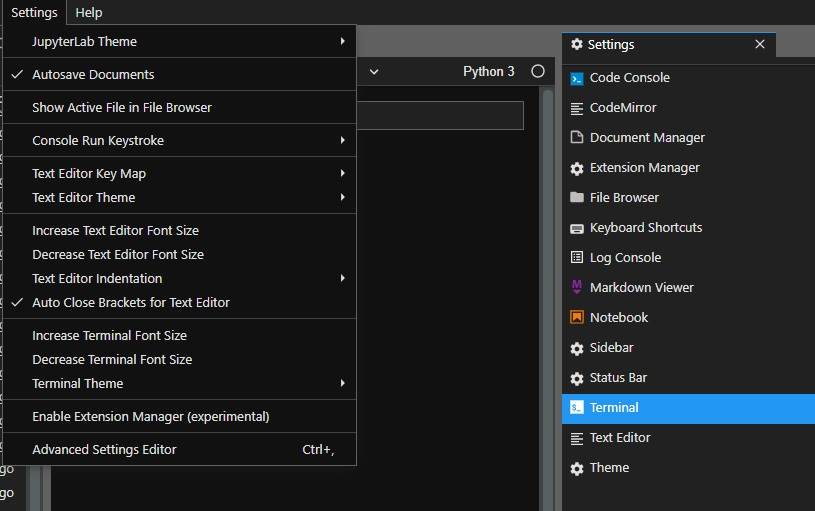
\includegraphics[width=15cm]{settings.jpg}
    \caption{Settings window}
    \label{fig:configuration}
\end{figure}

\section{Advanced Usage}

This section goes over how to use multiple programming languages in Jupyter\index{jupyter} and how to connect to your Jupyter Lab instance remotely.

\subsection{Multiple Kernels}

Adding a Kernel in Jupyter enables you to program with another programming language, such as R\index{r} or Scala\index{scala}.
Up to this point, we have been working with the Python kernel\index{python} which enables you to make python notebooks. The ability to use multiple kernels is useful for education and having cohesion within one IDE\index{IDE}.

You can view a complete list of kernels can be found on Jupyter's Github wiki.\footnote{\url{https://github.com/jupyter/jupyter/wiki/Jupyter-kernels}}

\begin{figure}[h!]
    \centering
    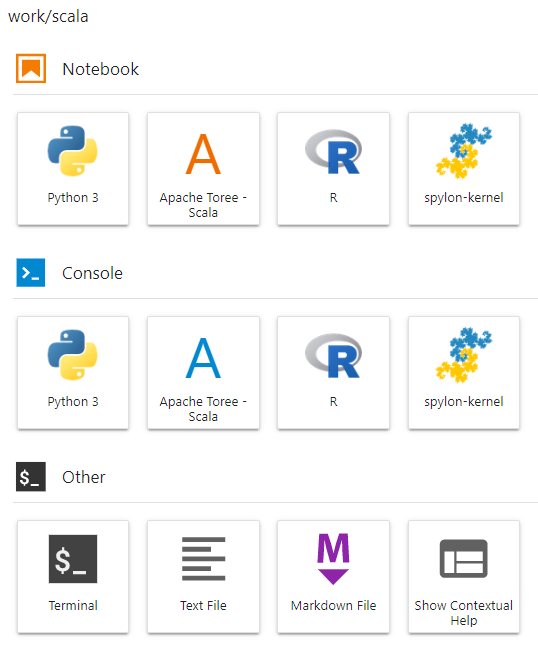
\includegraphics[width=50mm]{exampleKernels.PNG}
    \caption{Example of multiple kernels installed}
    \label{fig:multKernels}
\end{figure}

Figure 6 shows an example of what your launcher would look like with multiple kernels installed.

The most common way to install a kernel is by using the Anaconda\index{anaconda} prompt -- pip\index{pip} support is limited here.
Once you start adding multiple kernels, it is best if you start running Jupyter Lab through Docker\index{docker} because it would make porting it to another computer easier. A popular Docker Jupyter lab instance with Scala, Python, and R can be found on Jupyter's Docker hub profile\footnote{\url{https://hub.docker.com/u/jupyter/}}.

\subsection{Remote Connection}

If you have a firewall, Jupyter Lab will only be reachable on your
local machine at "localhost:8888". 
However, it is possible to connect to Jupyter Lab from remote computers. 
Remote access is helpful since it enables multiple people to connect to the same Jupyter instance. This would also save you resources on your local machine so you can program on a lightweight chrome-book that would not be able to run a full IDE\index{IDE} like Pycharm\index{pycharm}.

The first step to enable remote host would be to set a password that you can connect to the notebook using. You can set a password that you use to log into the website by executing the following command in a terminal:

\begin{lstlisting}
jupyter notebook password
\end{lstlisting}

The second step would be to launch the Jupyter Lab instance in a headless environment -- it never launches a web browser. 
A headless environments means that you never launch a GUI and it operates solely as a console application. 

\begin{lstlisting}
jupyter lab --no-browser --port=6000
\end{lstlisting}

The final step is to connect to the Jupyter Lab instance from your
remote computer.
The easiest way to do this is via a local port forward in SSH\index{ssh}. 
The command at listing 1 forwards all of the traffic from your local machine to a specific port on a remote computer over a SSH connection.
The main benefit of SSH is that all the traffic over the connection is encrypted.

Figure 7 shows an overview of what the network architecture looks like.

\newpage

\begin{lstlisting}[caption=SSH command for local port forwarding]
ssh -L 6000:localhost:6000 user@remote-host
\end{lstlisting}

\begin{figure}[h!]
    \centering
    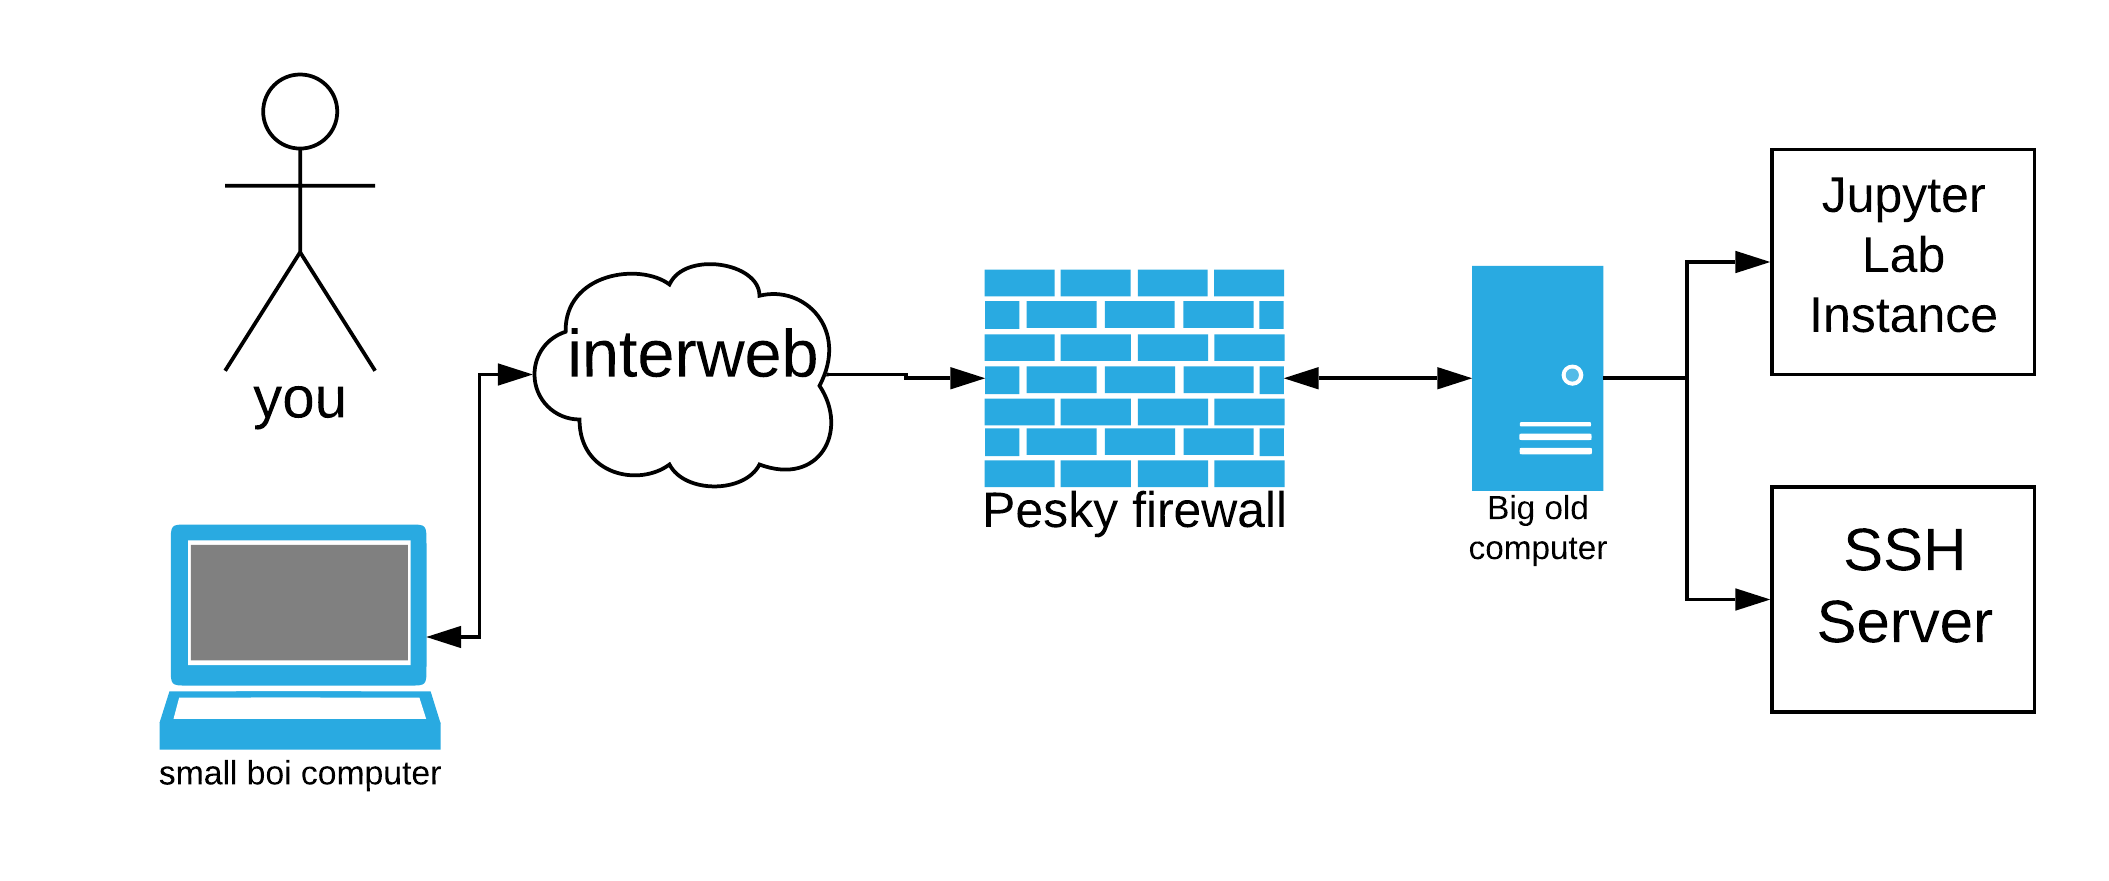
\includegraphics[width=15cm]{remoteJupyter.png}
    \caption{Network Overview}
    \label{fig:jupyter_server}
\end{figure}

After you execute the command above on your remote computer, you
will be able to access your Jupyter Lab instance at "localhost:6000" even though it is only running on the remote computer at port 6000.

\newpage

\section{Glossary}

\begin{itemize}[label={}]
\item {\bf Anaconda}: Anaconda is a package manager for the R and Python languages aimed towards data science" \footnote{\url{ https://www.anaconda.com}}.\index{anaconda}\\
\item {\bf IDE}: Interactive Development Environment-- some popular IDEs are Pycharm, Netbeans, and Visual Studio.\index{IDE}\\
\item {\bf Jupyter}: Nonprofit organization created to "develop open-source software, open-standards, and services for interactive computing across dozens of programming languages" \footnote{\url{ https://jupyter.org/}}.\index{jupyter}\\
\item {\bf JVM}: Java Virtual Machine\index{ssh}\\
\item {\bf Markdown(MD)}: Lightweight markup-language -- used to define layout and style for a document  \footnote{\url{https://en.wikipedia.org/wiki/Markdown}}.\index{markdown}\\
\item {\bf pip}: Tool for installing and managing python packages \footnote{\url{ https://pypi.org/project/pip/}}.\index{pip}\\
\item {\bf Pycharm}: A popular versatile Python IDE developed by \href{https://www.jetbrains.com/}{Jetbrains}.\index{IDE}\\
\item {\bf Python}: High-level interpreted, general purpose programming language \footnote{\url{ https://www.python.org/}}.\index{python}\\
\item {\bf R}: Programming language for statistical computing and graphics \footnote{\url{ https://www.r-project.org/}}.\index{r}\\
\item {\bf Scala}: General purpose functional programming language that runs on the JVM \footnote{\url{ https://scala-lang.org/}}.\index{scala}\\
\item {\bf SSH}: Secure Socket Shell -- used in connecting to a remote computer over a encrypted channel.\index{ssh}\\

\end{itemize}

\newpage

\section{References}

\begin{enumerate}
\item
\url{https://jupyter.org/}
\item
\url{https://www.python.org/}
\item
\url{https://en.wikipedia.org/wiki/Markdown}
\item
\url{https://pypi.org/project/pip/}
\item
\url{https://scala-lang.org/}
\item
\url{https://www.r-project.org/}
\item
\url{https://www.jetbrains.com/}
\end{enumerate}

\newpage

%\section{Index}
\printindex
% outputs its own heading, which does not match the sections

\end{document}